\documentclass[10pt]{article}
\usepackage[english]{babel}
\usepackage{url}
\usepackage{graphicx}
\usepackage{lscape}
\usepackage{float}
\usepackage{hyperref}
\usepackage{rotating}
\usepackage{listings}
\usepackage{multirow}
\usepackage{todonotes}
\usepackage{verbatim}
\usepackage{cite}
\graphicspath{ {./figures/} }

\usepackage[a4paper, left=3.5cm, right=3.5cm, top=4cm, bottom=3cm]{geometry}

\makeatletter
\renewcommand\paragraph{\@startsection{paragraph}{4}{\z@}%
            {-2ex\@plus -1ex \@minus -.25ex}%
            {1.ex \@plus .25ex}%
            {\normalfont\normalsize\bfseries}}
\makeatother
\setcounter{secnumdepth}{4} 
\setcounter{tocdepth}{4}   

\begin{document}

% HEADER PAGE
\begin{titlepage}
   \begin{center}
       \vspace*{1cm}
       {\fontsize{17}{16}\selectfont\textbf{Model-Driven Software Engineering Assignment}}

       \vspace{0.5cm}
        Model-Driven Software Engineering
            
       \vspace{1.5cm}

       \textbf{Group 2:}\\
       \textbf{Fábio Araújo de Sá (up202007658@up.pt)}\\
       \textbf{Filipe Rodrigues Fonseca (up202003474@up.pt)}\\
       \textbf{Lourenço Alexandre Correia Gonçalves (up202004816@up.pt)}\\
       \textbf{Pedro Pereira Ferreira (up202004986@up.pt)}\\
       \vfill
            
       
\includegraphics[width=0.6\textwidth]{imgs/FEUP.png}
        
       \vspace{2cm}
            
       November 2024
            
   \end{center}
\end{titlepage}

\tableofcontents
\clearpage

\section{Introduction}

This project aims to explore techniques and technologies of Model-Driven Software Engineering (MDSE), which can be applied to automate parts of the development of applications on low-code platforms \cite{brambilla2017mdse}. These platforms seek to simplify development by allowing the creation of complex solutions without the need for direct programming.

Throughout this project, we explored the different phases of constructing a pipeline that enables the transformation of ER Models into SQL code. To achieve this, we designed and implemented metamodels representing both ER models and Relational models, and these were validated through specific test cases. Afterward, constraints for the model-to-model transformation were created. Finally, a model-to-text transformation was performed to obtain valid and executable SQL code derived from the initial model.

At every stage, the main challenges were identified, and the decisions made were justified.

\section{Tools and Technologies}

For the implementation of the project, we used the following tools and technologies:

\begin{itemize}

    \item \textbf{Eclipse\footnote{https://www.eclipse.org}}: an integrated development environment (IDE) that served as the main platform for development and the integration of other tools;
    
    \item \textbf{Ecore\footnote{https://wiki.eclipse.org/Ecore/}}: part of the Eclipse Modeling Framework (EMF), which allows the creation, manipulation, and validation of metamodels. It was used to define the formal languages for the source and target models;

    \item \textbf{XMI\footnote{https://www.omg.org/spec/XMI/}}: XML Metadata Interchange, is a standard for exchanging metadata information via Extensible Markup Language.

    \item \textbf{Object Constraint Language (OCL)\footnote{https://projects.eclipse.org/projects/modeling.mdt.ocl}}: used to define integrity constraints on metamodel instances, ensuring that the models adhere to all the necessary rules and consistencies during transformations;
    
    \item \textbf{OCLinEcore\footnote{https://wiki.eclipse.org/OCL/OCLinEcore}}: is an extension that integrates OCL expressions into Ecore models, allowing for more expressive constraints and operations within models;
    
    \item \textbf{Atlas Transformation Language (ATL)\footnote{https://eclipse.dev/atl/}}: used for applying model-to-model (M2M) transformations, enabling the conversion of more abstract models (such as ER models) to domain-specific models (such as relational models);
    
    \item \textbf{Acceleo\footnote{https://projects.eclipse.org/projects/modeling.acceleo}}: a tool for applying model-to-text (M2T) transformations, used to generate code from the final models, allowing, in this case, the generation of valid SQL code.
    
\end{itemize}

These tools enabled the automation of the pipeline developed from the proposed models and domains. The use of metamodeling stategies ensured the validation of the models, their transformation, and the appropriate output.

\section{Modeling Domain Analysis}

At this stage, we analyzed the domain to define the source and target models that will be used throughout the project. The analysis of one concrete example helped to delineate the scope of the project, ensuring that our metamodels capture all the concepts covered in the domain and validate each one appropriately.

\subsection{Domain}

To understand the domain and define the project's boundaries, we analyzed practical one example of two types of models commonly used as the foundation for generating SQL code: Entity-Relationship (ER) models and Relational models. This example guided the development of the metamodels and also served as test cases in the subsequent phases.

\subsubsection{ER Model}

The Entity-Relationship (ER) model\footnote{https://en.wikipedia.org/wiki/Entity–relationship-model}\footnote{https://www.geeksforgeeks.org/introduction-of-er-model/} is a conceptual approach to data modeling that visually represents the logical structure of an information system and the relationships between the data within that system. Taking the concrete example of a chain of gyms with equipment, where each gym can have multiple customers, and them can have some characteristics in the system, we can derive the ER model as represented in Figure \ref{figure1}:

\begin{center}
    \begin{figure}[H]
        \centering
        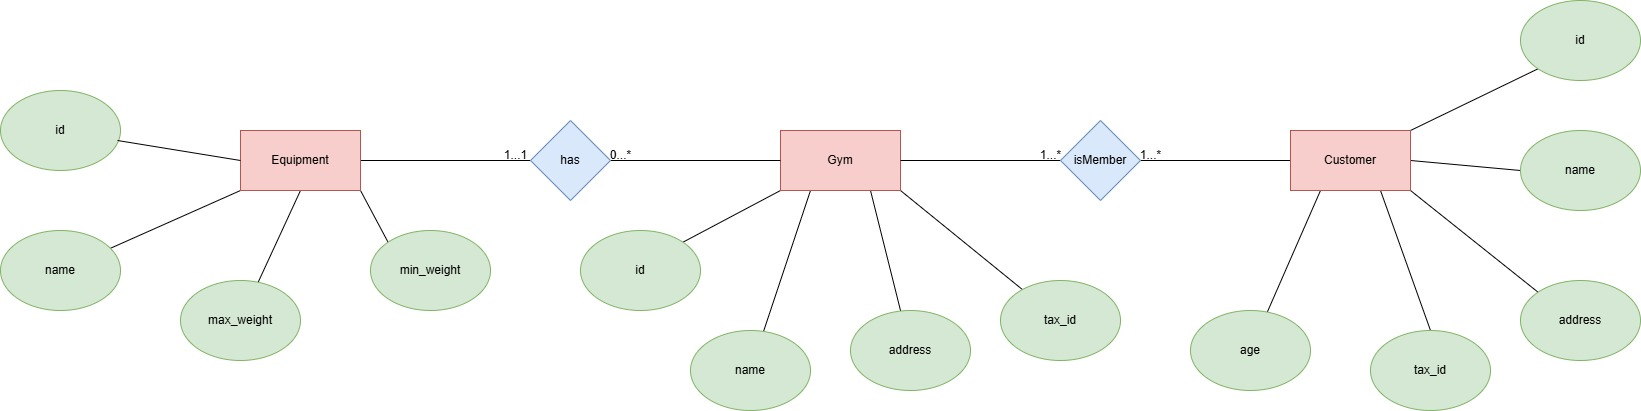
\includegraphics[width=1.0\textwidth]{imgs/er-model.png}
            \caption{Gym ER Model example}
        \label{figure1}
    \end{figure}
\end{center}

In this example, as well as in similar models, it is essential to ensure the existence of:

\begin{itemize}
    \item Entities;
    \item Attributes with associated entities;
    \item Relationships with various multiplicities (one-to-one, one-to-many, many-to-many) between entities.
\end{itemize}

For the sake of simplifying future validations, the system will only be designed to handle attributes of type string and integer. Thus, the model is considered valid if it allows the creation of attributes with these types, entities with attributes, and relationships of any cardinality between the entities in the system.

\subsubsection{Relational Model}

The Relational Model\footnote{https://www.geeksforgeeks.org/relational-model-in-dbms/} is a data modeling approach that organizes information into tables, or relations, where each table consists of columns (its attributes) and rows (the actual data). Unlike the Entity-Relationship (ER) model, which is more conceptual and visual, the relational model focuses on the effective implementation of data in Database Management Systems (DBMS), thereby aligning more closely with the ultimate goal of generating SQL code. Using the previous example of the chain of gyms, a translation of the above into a Relational Model can be represented as shown in Figure \ref{figure2}:

\begin{center}
    \begin{figure}[H]
        \centering
        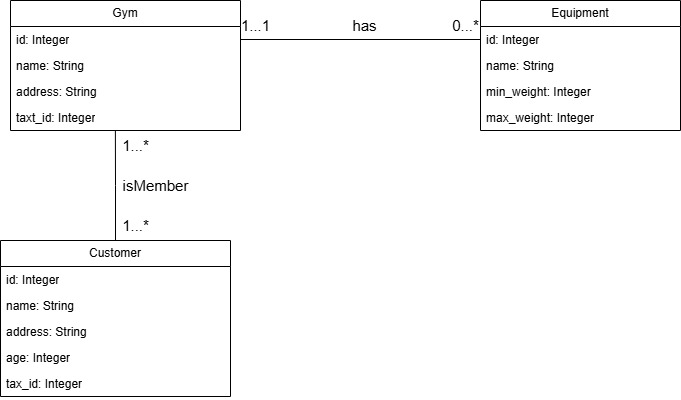
\includegraphics[width=0.9\textwidth]{imgs/relational-model.png}
            \caption{Gym Relational Model example}
        \label{figure2}
    \end{figure}
\end{center}

Thus, the relational models to be manipulated will include:

\begin{itemize}

    \item Varied multiplicities between tables (one-to-one, one-to-many, many-to-many);
    
    \item Tables with multiple attributes, including the necessary primary and foreign keys;
    
    \item Relationships between tables, with the corresponding keys and associated multiplicities.
    
\end{itemize}

In the project, generalizations between tables, self-dependencies, and composite foreign keys were not considered. Any model with these functionalities in our project must be invalidated in the corresponding metamodel.

\subsubsection{SQL Code}

The final objective of the project is to ensure a standard, valid Structured Query Language (SQL) code that can be executed, for example, in one database engine like PostgreSQL\footnote{https://www.postgresql.org}. For the final code to be considered valid, the following requirements must be met:

\begin{itemize}

    \item The output file must have the \textbf{.sql} extension;
    
    \item There must be a schema definition, \textbf{CREATE SCHEMA}, in the file header;
    
    \item There must be \textbf{DROP TABLE} statements in the header of the file to ensure the database can be reset without key collisions or duplicate IDs;
    
    \item The definition of each table, attributes and relationships;
    
    \item The explanation of primary keys and foreign keys, if available.
    
\end{itemize}

The code snippet in Annex \ref{Annex1} demonstrates the expected result from the gym example. It is important to note that in SQL, all generated tables explicitly define their primary keys and, where applicable, the corresponding foreign keys. For standardization purposes, and since not all database engines operate with the same keywords, implementations of internal primary keys using keywords such as \textbf{AUTOINCREMENT}, \textbf{ROWID} or \textbf{SERIAL} have been excluded. Instead, it is assumed that all keys are inserted manually. Conversely, to ensure final code validation in database engines, the \textbf{NOT NULL} constraint should be applied to all primary and foreign key declarations.

\subsection{Concepts}

After defining the problem domain and to gain a more high-level perspective for preparing the corresponding metamodels, the key concepts of both models were gathered and explored.

In the case of the ER model, the following components were identified:

\begin{itemize}

    \item \textbf{Entity}: represents a distinct object or concept within the system;
    
    \item \textbf{Attribute}: defines the characteristics of an entity;
    
    \item \textbf{Relation}: represents the connections between two or more entities.
    
\end{itemize}

Regarding constraints, it is important to note that each entity can have multiple attributes, and each attribute belongs to only one entity. On the other hand, a relation is the result of the connection between a pair of entities. The multiplicity of each relation can be one-to-one, one-to-many, or many-to-many.

In contrast to the previous model, the Relational Model includes other concepts that are more closely aligned with the properties found in SQL:

\begin{itemize}

    \item \textbf{Table}: corresponds to the entity in the previous model;
    
    \item \textbf{Column}: corresponds to the attribute of each entity;
    
    \item \textbf{Primary Key}: column that uniquely identifies each record in the table;
    
    \item \textbf{Foreign Key}: column in a table that references another existent table.
    
\end{itemize}

In terms of constraints, we can conclude that a table in this Relational Model has columns, and each column belongs to a single table. Additionally, there is only one primary key per table, but multiple foreign keys can exist, provided they have a valid reference to another table.

Each of these identified components, along with their constraints, was implemented using Ecore classes. In the following section, we will express the process of creating the corresponding Metamodels.

\section{Metamodel Design}

Having established the key components and constraints of both the Entity-Relationship model and the Relational model, we were ready to delve into the design of the metamodels. Using Ecore, we defined the classes and relationships that encapsulate the identified components, ensuring that they adhere to the constraints we had outlined.

\subsection{ER Metamodel}

The ER Metamodel was formed by:

\begin{itemize}

    \item \textbf{Entity}: has a ename (EString) and can be associated with multiple Attributes;
    
    \item \textbf{Attribute}: has a aname (EString), a data type (EString), isIdentifier (EBoolean) and a correspondent Entity;
    
    \item \textbf{Relation}: has a unique rname (EString) and a multiplicity, defined by two integer pairs (EInt) representing the lower and upper bounds, which describe the number of instances of each entity that can participate in the relationship.
    
\end{itemize}

For many-to-many multiplicity cases, we considered the standard Ecore value: -1. To ensure Ecore compatibility, we added an \textbf{Model} component that can contain all entities and relationships in the system and has a name (EString). Since ER models do not inherently indicate the potential primary keys of entities, and this information is crucial for defining the future relational model, we chose to add a boolean attribute, \textbf{isIdentifier}, which marks attributes that, being unique and non-null, can independently identify the entity within the system.

The Ecore framework generated a visual representation of the metamodel. The Figure \ref{figure3} provides an overview of how entities, attributes, and relations are interconnected:

\begin{center}
    \begin{figure}[H]
        \centering
        
\includegraphics[width=1.0\textwidth]{imgs/er-metamodel.jpeg}
            \caption{ER Metamodel}
        \label{figure3}
    \end{figure}
\end{center}

\subsection{Relational Metamodel}

The Relational Metamodel was formed by:

\begin{itemize}

    \item \textbf{Schema}: has a name (EString) and can be associated with all system Tables;
 
    \item \textbf{Table}: has a name (EString) and can be associated with multiple Columns;
    
    \item \textbf{Column}: has a name (EString), a data type (EString), isNullable (EBoolean), isUnique (EBoolean), and has a correspondent Table;
    
    \item \textbf{Primary Key}: a column that uniquely identifies each record in the table;
    
    \item \textbf{Foreign Key}: a column in one table that creates a link to the primary key of another table, establishing a relationship between the two tables;
    
\end{itemize}

The Ecore framework generates a visual representation of the Relational metamodel, illustrating the relationships between tables, columns, and keys. The Figure \ref{figure4} clarifies how the components interact within the relational structure:

\begin{center}
    \begin{figure}[H]
        \centering
        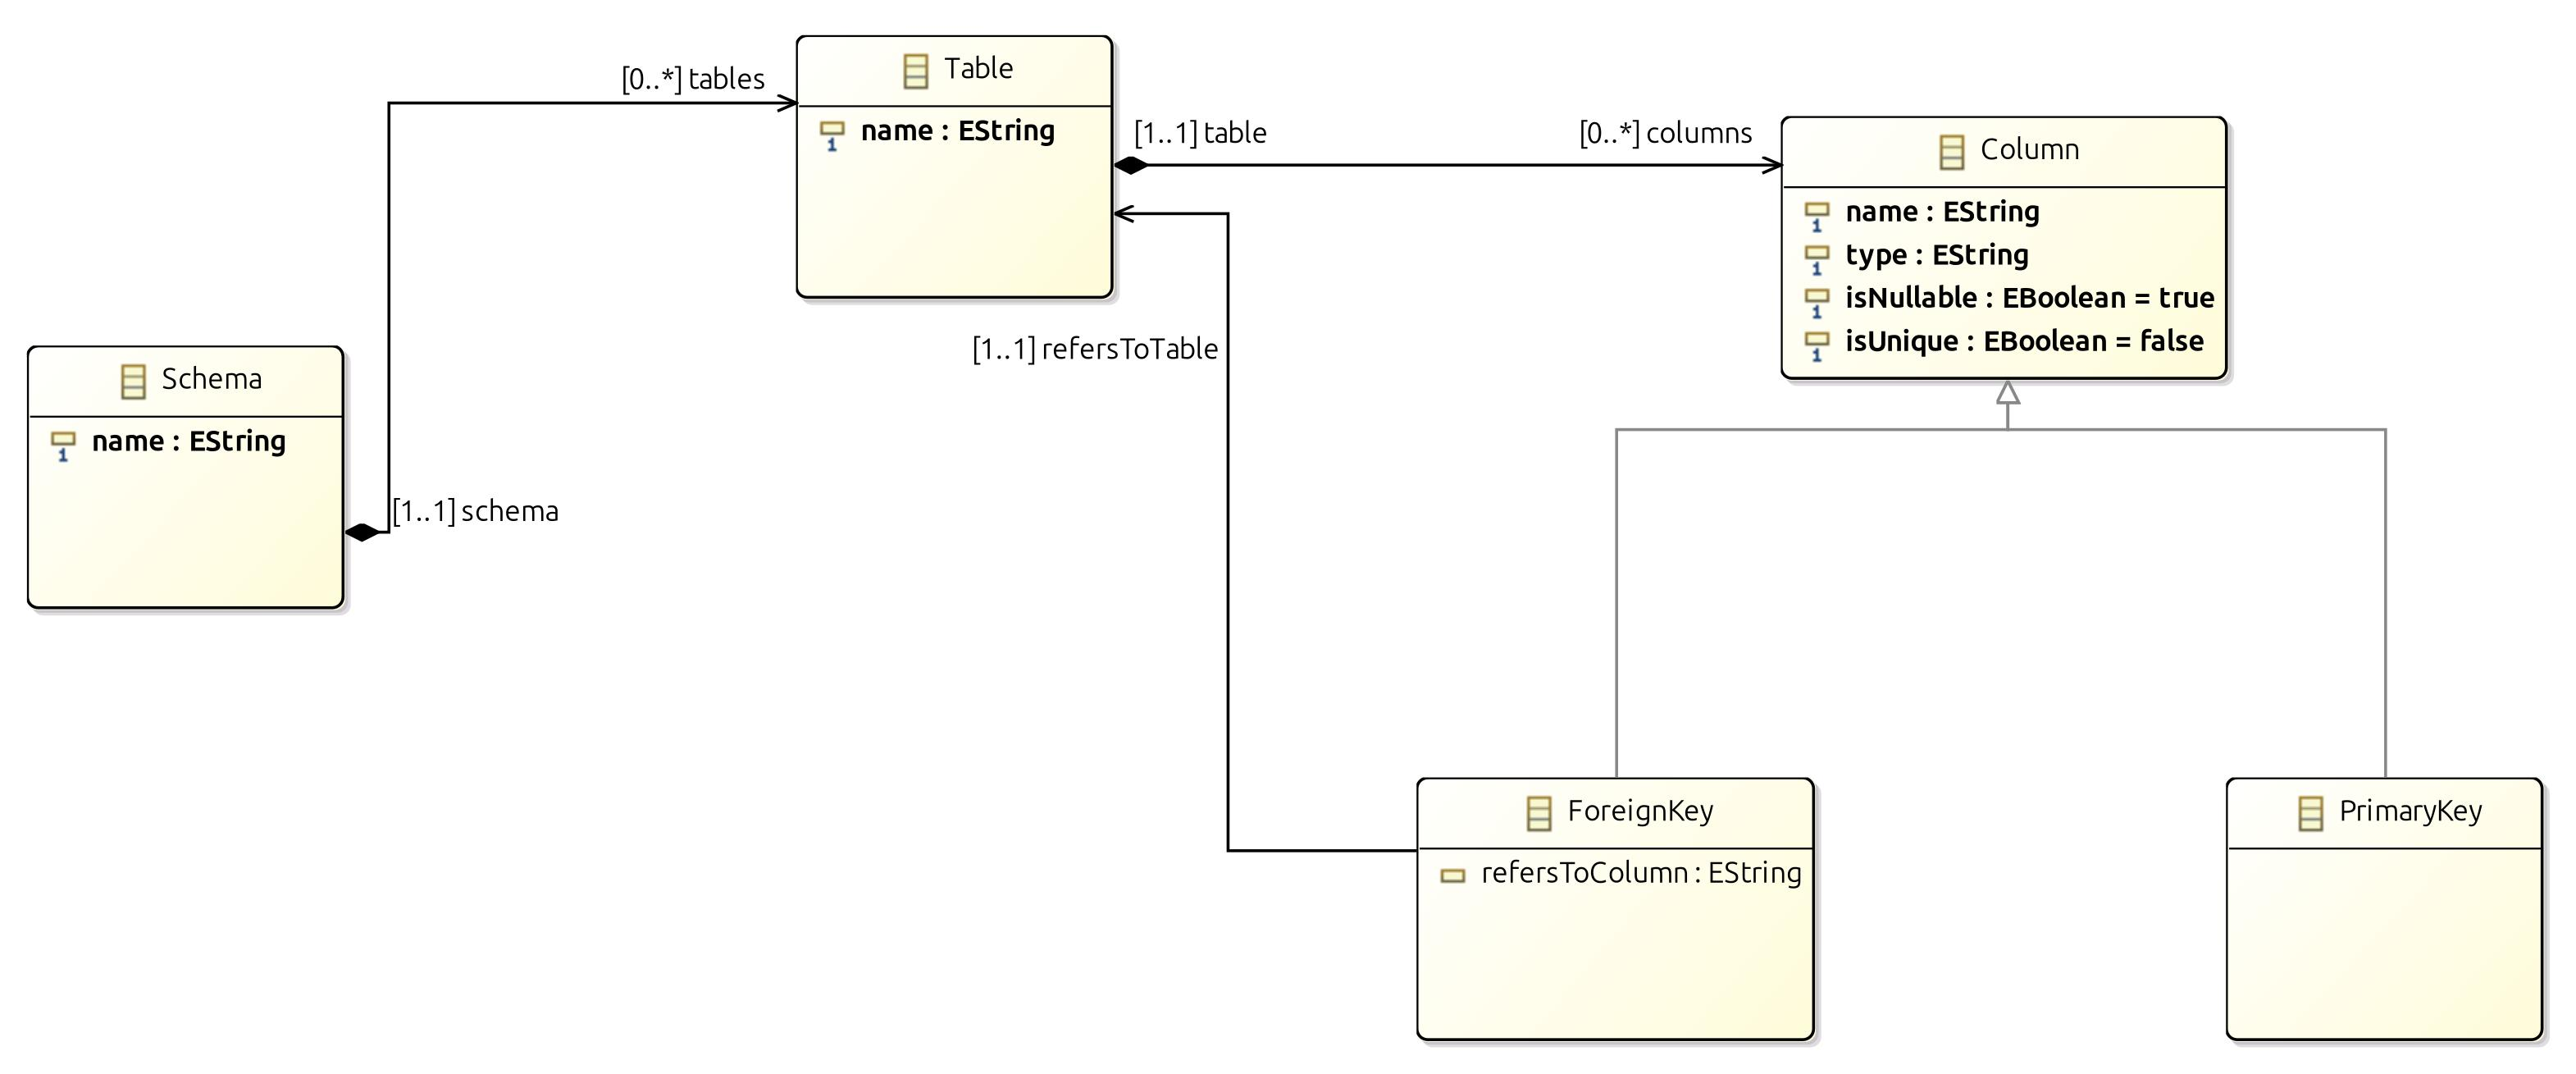
\includegraphics[width=1.0\textwidth]{imgs/relational-metamodel.png}
            \caption{Relational Metamodel}
        \label{figure4}
    \end{figure}
\end{center}

Note that the generalization of Column into Primary Key and Foreign Key is an incomplete and disjoint generalization. In terms of implementation, three attributes were added to Column:

\begin{itemize}

    \item \textbf{isPrimaryKey}: (boolean - EBoolean), which defaults to False and indicates whether this column is a primary key in the corresponding table;
 
    \item \textbf{isForeignKey}: (boolean - EBoolean), which defaults to False and indicates whether this column is a foreign key in the corresponding table;
    
    \item \textbf{refersToColumn}: (string - EString), which defaults to Null and represents the name of the referenced table if this column is a foreign key.
    
\end{itemize}

Multiplicities do not need to be explicitly defined in the metamodel, as they are expressed by the existence of foreign keys between tables or by adding new tables, which will be ensured by the model-to-model transformation discussed in later sections.

\section{Metamodel Constraints}

In this section, we explored the constraints and validations of the metamodels. This process involved applying various integrity constraints and invariants to ensure that the generated models adhere to the defined rules. The metamodels were subjected to various tests that checked each of the programmed constraints. We used the Object Constraint Language (OCL) within the Ecore framework to express these constraints, providing a mechanism for validating the integrity of our inputs.

\subsection{Constraints}

To maintain data integrity throughout the modeling process, we implemented the following OCL constraints:

\begin{itemize}

    \item \textbf{C1}: The model/schema must contain entities/tables with unique, not-empty names;

    \item \textbf{C2}: All entities/tables must have attributes/columns with unique, not-empty names;
    
    \item \textbf{C3}: All entities/tables must have an identifier/primary key;
    
    \item \textbf{C4}: The lower multiplicity must be less than or equal to the upper bound, and both values must be non-negative;
    
    \item \textbf{C5}: The primary key must be unique and not null;
    
    \item \textbf{C6}: Columns in tables that are foreign keys must refer to an existing table in the system, other than itself;

    \item \textbf{C7}: No schema, table or column name can be an SQL Reserved Word;

    \item \textbf{C8}: The column type must a valid SQL data type;

    \item \textbf{C9}: The column referenced by a foreign key must be UNIQUE;

    \item \textbf{C10}: The referenced table of a foreign key must have the referenced column;

    \item \textbf{C11}: The column type of a foreign key must be of the same type as the one it references.

    
    
\end{itemize}

Constraints C1 to C3 were implemented in both metamodels, while C4 applies only to the ER Metamodel. Constraints C5 to C11 are specific to the Relational Metamodel. The implementation details can be found in the \textbf{er.ecore} and \textbf{relational.ecore} files attached to the submission.

These constraints ensure that the models are well-defined and that the relationships between various components are valid, thereby preserving the integrity of the final database structure.

\subsection{Validation}

The validation of the modeling constraints involved encoding various test cases to verify compliance with the metamodels. This step was essential to confirm that the implemented constraints functioned as intended and that the models adhered to the specifications set in the metamodel design.

The project submission includes a tests folder containing various test cases. For instance, the file \textbf{test1-er.xmi} was used as input for the ER metamodel to test Constraint 1 (C1), while \textbf{test5-relational.xmi} served as input for the Relational Metamodel to test Constraint 5 (C5). Additional files, such as \textbf{gym-er.xmi}, \textbf{gym-relational.xmi}, \textbf{complex-er.xmi}, and \textbf{complex-relational.xmi}, represent valid models for a gym example in both metamodels, as well as a more complex but still valid example. Table \ref{constraints-validation} summarizes the expected and obtained results for each test case following validation attempts.

\begin{table}[H]
\begin{tabular}{|c|c|c|c|}
\hline
\textbf{\begin{tabular}[c]{@{}c@{}}Targeted\\Constraint\end{tabular}} & \textbf{Test File}                              & \textbf{Expected Result} & \textbf{Obtained Result} \\ \hline
\textit{C1}         & test1-\textless{}er, relational\textgreater{}.xmi   & Fail                     & Fail                     \\ \hline
\textit{C2}         & test2-\textless{}er, relational\textgreater{}.xmi   & Fail                     & Fail                     \\ \hline
\textit{C3}         & test3-\textless{}er, relational\textgreater{}.xmi   & Fail                     & Fail                     \\ \hline
\textit{C4}         & test4-er.xmi                                        & Fail                     & Fail                     \\ \hline
\textit{C5}         & test5-relational.xmi                                & Fail                     & Fail                     \\ \hline
\textit{C6}         & test6-relational.xmi                                & Fail                     & Fail                     \\ \hline
\textit{C7}         & test7-relational.xmi                                & Fail                     & Fail                     \\ \hline
\textit{C8}         & test8-relational.xmi                                & Fail                     & Fail                     \\ \hline
\textit{C9}         & test9-relational.xmi                                & Fail                     & Fail                     \\ \hline
\textit{C10}         & test10-relational.xmi                                & Fail                     & Fail                     \\ \hline
\textit{C11}         & test11-relational.xmi                                & Fail                     & Fail                     \\ \hline
\textit{All}         & gym-\textless{}er, relational\textgreater{}.xmi     & Success                  & Success                  \\ \hline
\textit{All}         & complex-\textless{}er, relational\textgreater{}.xmi & Success                  & Success                  \\ \hline
\end{tabular}
\caption{Validation Results for Metamodel Constraints}
\label{constraints-validation}
\end{table}

Full coverage of all constraints was achieved, ensuring the integrity of the generated ER and Relational metamodels.

\begin{comment}

\section{Model-to-Model Transformations}

In this section, we explored the transformation process from the Entity-Relationship model to the Relational model. This process involved applying various integrity constraints to ensure that the transformed models adhere to the defined rules. We used Atlas Transformation Language (ATL) within the Ecore framework to express these constraints, providing a mechanism for validating the integrity of our transformations.

https://www.geeksforgeeks.org/mapping-from-er-model-to-relational-model/

TODO

\section{Model-to-Text Transformations}

TODO

\end{comment}

\section{Conclusion}

In this phase, we successfully explored and implemented key techniques and technologies within Model-Driven Software Engineering to facilitate the automation of application development on low-code platforms. By designing and validating metamodels for both Entity-Relationship and Relational models, we established a solid foundation for understanding the essential components and constraints inherent in the modeling process. This groundwork clarified the relationships between entities, attributes, and relationships, ensuring the integrity and validity of the models throughout the project.

\section{Contributions}

In this phase, the group members have contributed equally for the project's development. As a result, it was given the same grade in percentage, so that its sum is 100\%, as shown on the list below:

\begin{itemize}

    \item \textbf{Fábio Sá}: 25\%;

    \item \textbf{Filipe Fonseca}: 25\%;
    
    \item \textbf{Lourenço Gonçalves}: 25\%;
    
    \item \textbf{Pedro Ferreira}: 25\%.
    
\end{itemize}

In qualitative terms, all the group members have contributed in the whole project process. In other words, every group member has helped with:

\begin{itemize}

    \item Modeling Domain Analysis;

    \item Modeling Language Design, contributing the development of ER and Relational models;

    \item Development of integrity constraints for the models;
    
    \item Models Testing;
    
    \item Writing the report.
    
\end{itemize}

\bibliographystyle{apalike}
\bibliography{references}

\newpage
\appendix 

\section{Annex} \label{Annex1}

\begin{lstlisting}[language=SQL]
CREATE SCHEMA Gyms;

DROP TABLE IF EXISTS Gym;
DROP TABLE IF EXISTS Customer;
DROP TABLE IF EXISTS Equipament;
DROP TABLE IF EXISTS isMember;

CREATE TABLE Gym (
    id INTEGER NOT NULL,
    name VARCHAR(255),
    address VARCHAR(255),
    tax_id: Integer,
    PRIMARY KEY (id)
);

CREATE TABLE Customer (
    id INTEGER NOT NULL,
    name VARCHAR(255),
    address VARCHAR(255),
    age INTEGER,
    tax_id: INTEGER,
    PRIMARY KEY (id) 
);

CREATE TABLE Equipament (
    id INTEGER NOT NULL,
    name VARCHAR(255),
    min_weight INTEGER,
    max_weight INTEGER,
    gym_id INTEGER NOT NULL,
    FOREIGN KEY (id) references Gym (id)
);

CREATE TABLE isMember (
    id INTEGER NOT NULL,
    client_id INTEGER NOT NULL,
    gym_id INTEGER NOT NULL,
    PRIMARY KEY (id),
    FOREIGN KEY (client_id) REFERENCES Client (id),
    FOREIGN KEY (gym_id) REFERENCES Gym (id)
);
\end{lstlisting}

\end{document}
